\section{Side by side comparison}
\label{sec:comparison}

In this section we compare both results side by side. Firstly, the output of the envelope detector (take note that the theoritcal analysis one is the plot in orange):
\begin{figure}[h]
    \centering
    \begin{subfigure}{0.23\textwidth}
        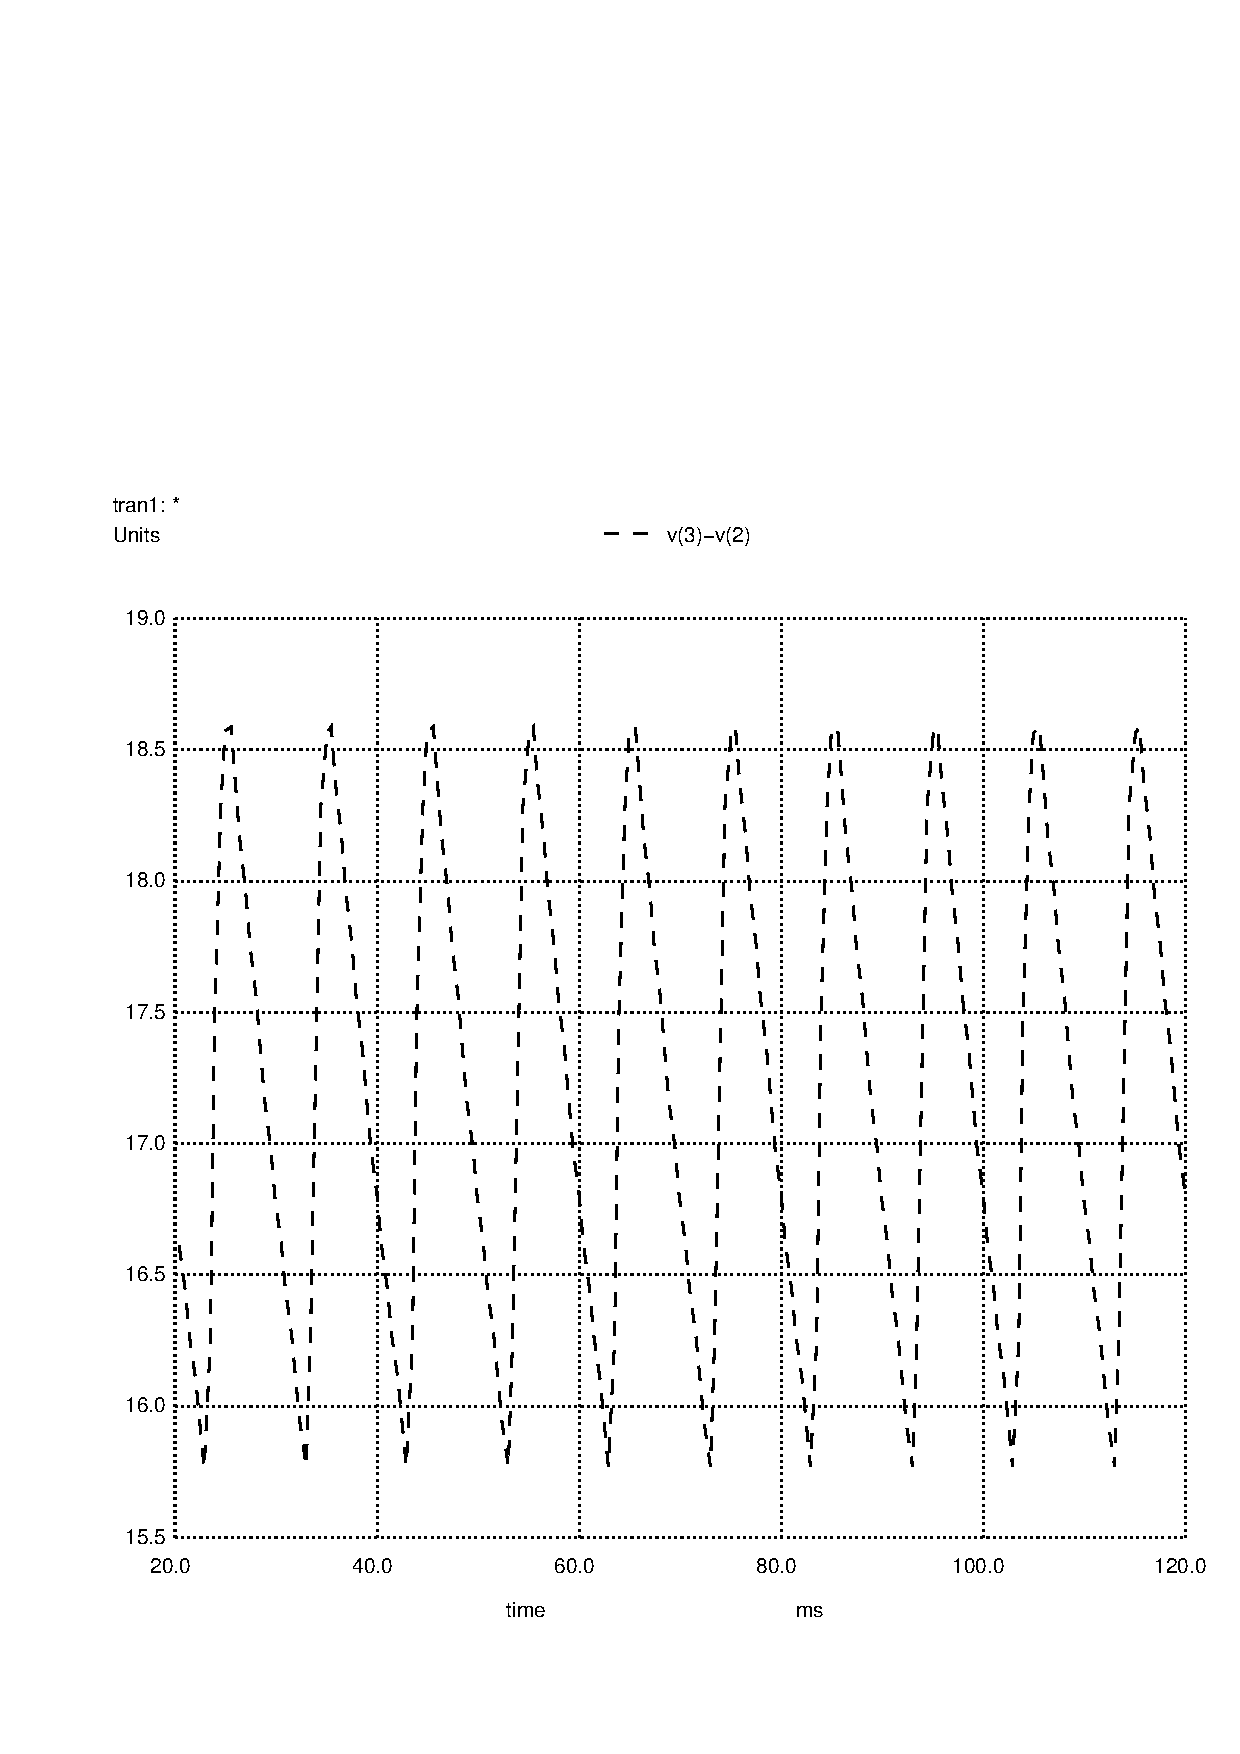
\includegraphics[width=\linewidth, clip]{solution2.pdf}
        \label{fig:envd1}
    \end{subfigure}
    \begin{subfigure}{0.23\textwidth}
        \includegraphics[width=\linewidth, clip]{venvlope.eps}
        \label{fig:envd2}
    \end{subfigure}
    \caption{\small Envelope detector output (left - simulation; right - theoretical )}
    \label{env_detector}
\end{figure}

\begin{figure}[h]
    \centering
    \begin{subfigure}{0.23\textwidth}
        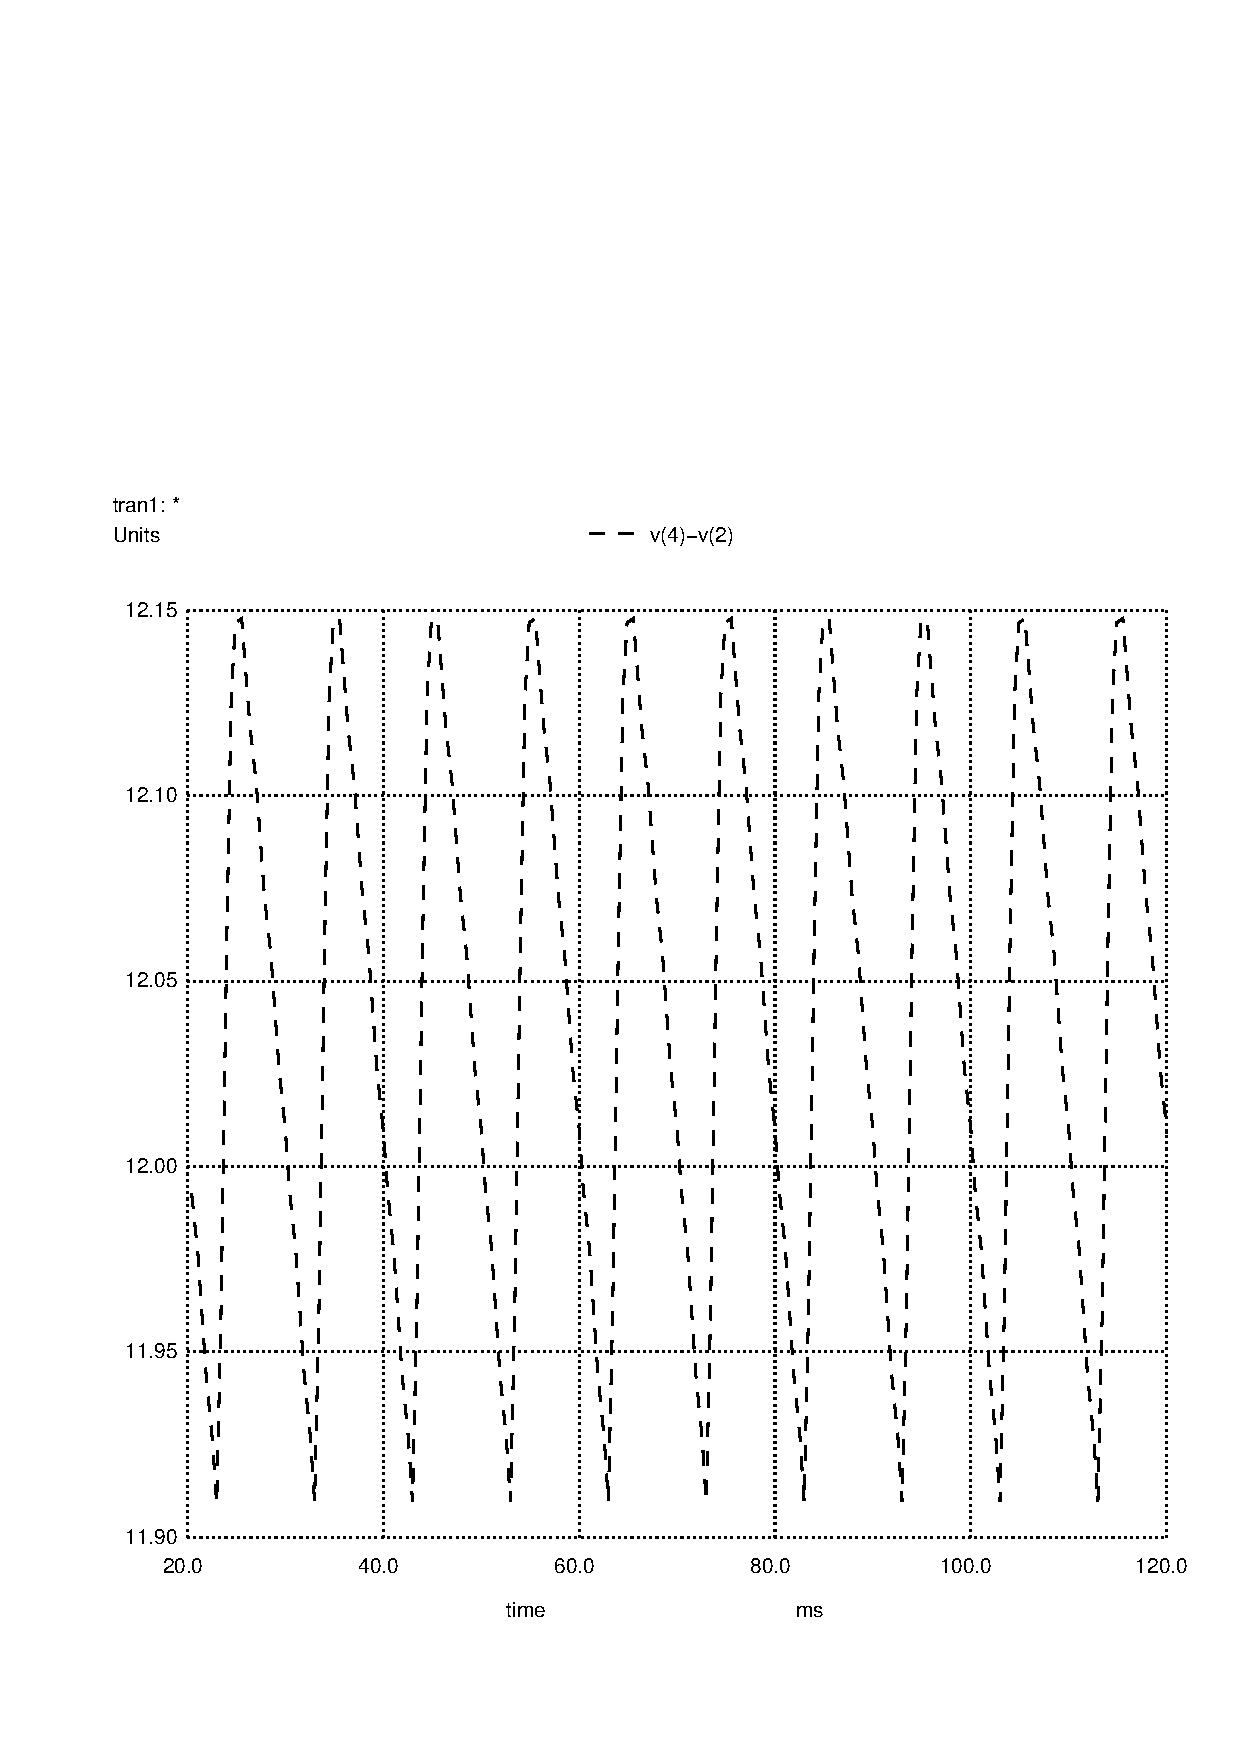
\includegraphics[width=\linewidth, clip]{solution1.pdf}
        \label{fig:voltr1}
    \end{subfigure}
    \begin{subfigure}{0.23\textwidth}
        \includegraphics[width=\linewidth, clip]{voltageRegulator.eps}
        \label{fig:voltr2}
    \end{subfigure}
    \caption{\small Voltage regulator output (left - simulation; right - theoretical )}
    \label{volt_reg}
\end{figure}

The shape of the graphs, both envelope detector and voltage regulator is similar, so we can concluse that both fullfill their purposes and the theoretical model used was good at predicting the general behaviour of the circuit. 
However, especially on the voltage regulator graphs, we can see some differences in the scale of the oscillations, that can be due to the different models used in our theoretical simulation, compared to ngspice.
We can quantify this diffetence with the values of the ripples. 

\begin{figure}[h]
    \centering
    \begin{subfigure}{0.23\textwidth}
        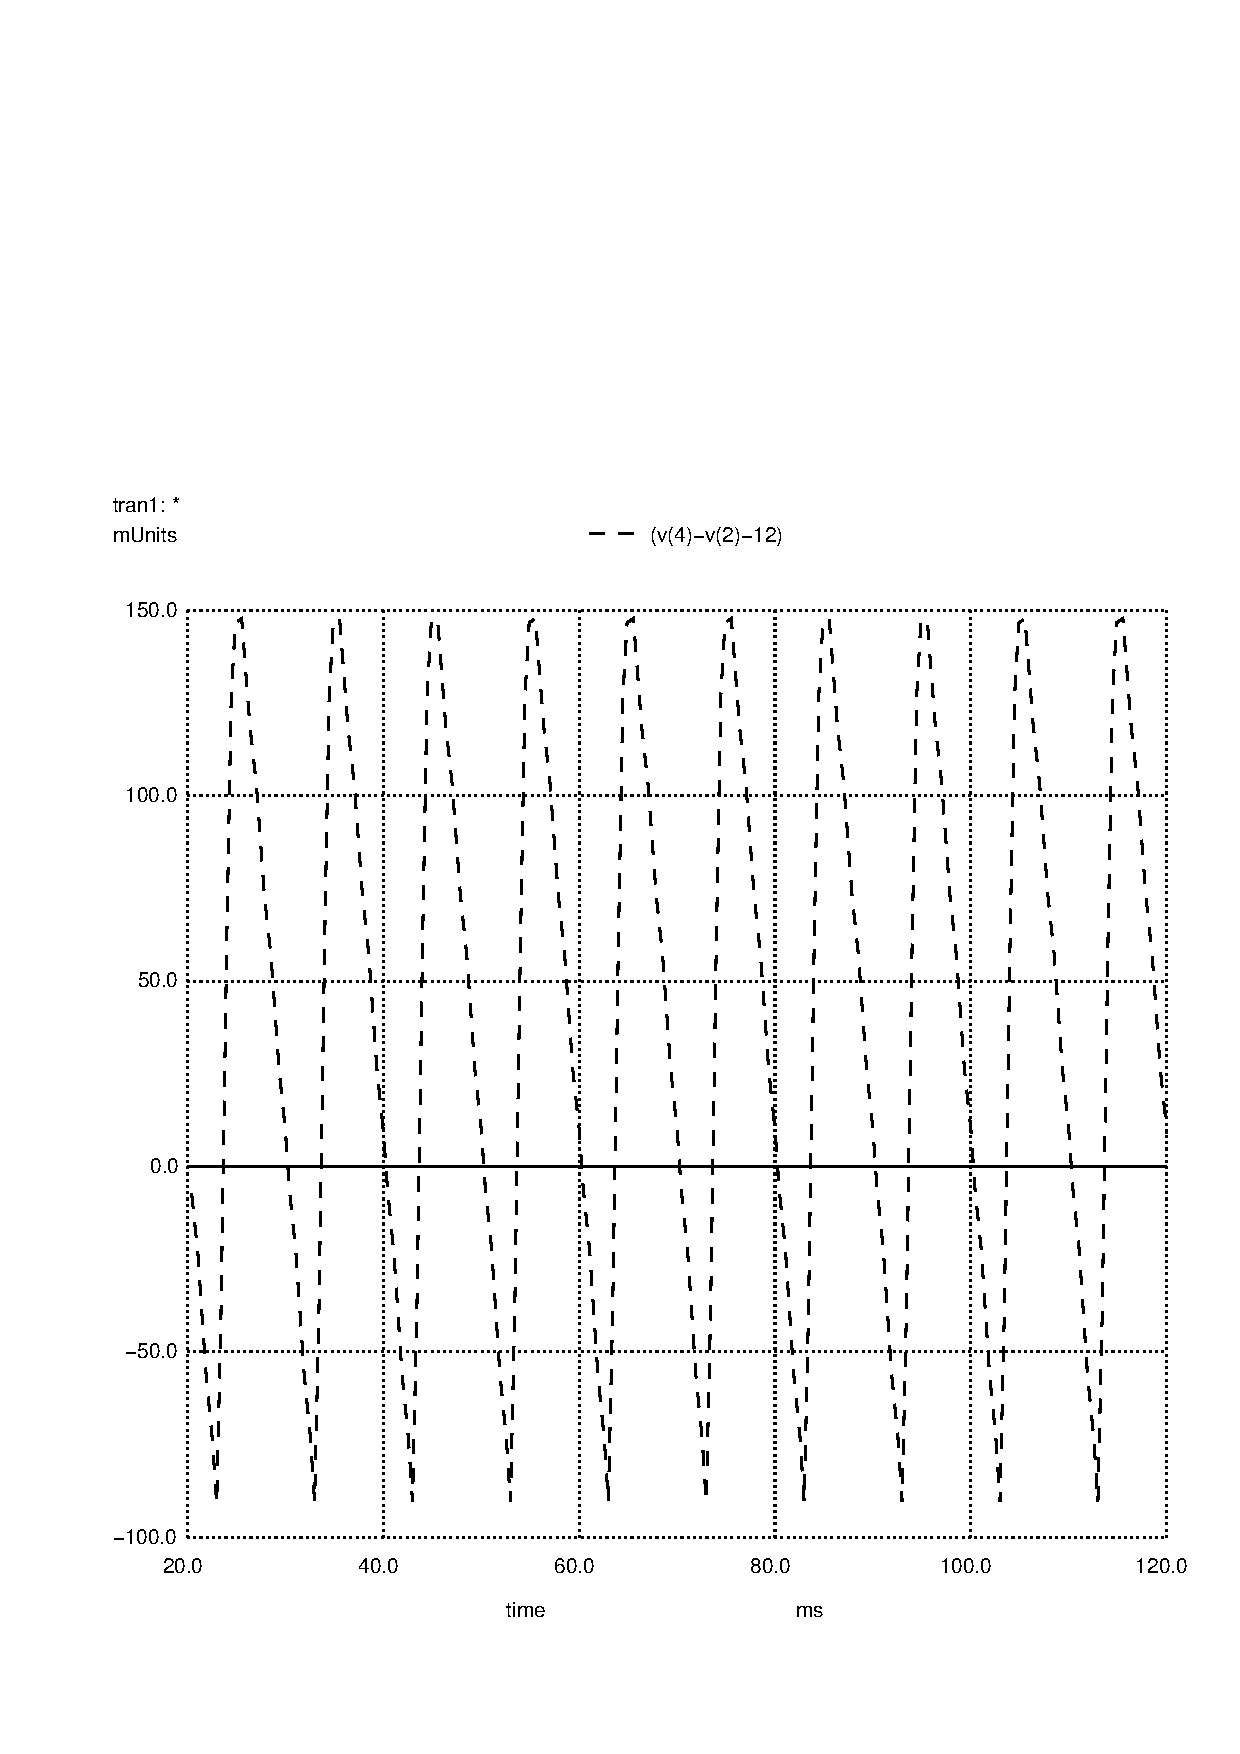
\includegraphics[width=\linewidth, clip]{solution12.pdf}
        \label{fig:output1}
    \end{subfigure}
    \begin{subfigure}{0.23\textwidth}
        \includegraphics[width=\linewidth, clip]{Deviation.eps}
        \label{fig:output2}
    \end{subfigure}
    \caption{\small $V_Out - 12$ - measure of the output DC deviation + AC component (left - simulation; right - theoretical )}
    \label{output_deviation}
\end{figure}

Once again, as in the previous graphs, the output deviation graph has a similar shape but a noticeable difference in scale, probably due to different models.


\begin{center}
\begin{tabular}{ |c|c|c| }
 \hline 

  & Simulation & Theoretical \\
  Ripple &  0.2391470  &  0.38944 \\ 

  \hline 

\end{tabular}
\end{center}

Thus we have obtained a 62\% error in the theoretical ripple. Which is a 
good indicator of the difference between the models used. 

\section{Conclusion}
\label{sec:conclusion}


The ultimate goal of this laboratory assignment, to analyse
the given circuit theoretically and using simulation, has been achieved, since
the simulation results matched the theoretical results with some accuracy.
The results were expected, as explained in the last section, because 
the models used to describe the components of the circuit, namely the diodes, 
in \textit{Ngspice} and in the theoretical analysis (\ref{sec:analysis}) are 
extremely different. Better results could have been obtained if other 
models for the behaviour of the diodes were used, for instance, the 
exponential model.

%\lipsum[1-1]
